% Slides made from MCIQ4memo.tex
% compile with  pdflatex MCIQ4slides.tex   (twice)
\documentclass[aspectratio=169,10pt]{beamer}
\usetheme{Boadilla}
\usecolortheme{beaver}
\usefonttheme[onlymath]{serif}
\setbeamertemplate{navigation symbols}{}
\setbeamertemplate{itemize items}[circle]
\setbeamercolor{block title}{bg=red!15,fg=darkred}
\setbeamercolor{block body}{bg=red!5}

\usepackage{amsmath,amssymb,graphicx,booktabs}

\renewcommand{\d}{\,\mathrm{d}}
\newcommand{\e}{\mathrm{e}}
\newcommand{\E}{\mathrm{E}}
\newcommand{\skappa}{\tilde\kappa}
\newcommand{\MC}{\texttt{MCIQ4.cpp}}
\newcommand{\ISIF}{\texttt{IQ4.cpp}}

\title[Monte Carlo for the VRTE]{A Monte Carlo method for the stratified VRTE}
\subtitle{system (4.9)--(4.10)--(4.11) of Chapter 4}
\author{O. Pironneau}
\date{\today}

\begin{document}

\begin{frame}\titlepage\end{frame}

%--------------------------------------------------------------------
\begin{frame}{The problem}
\small
For $z\in(0,Z)$, $\mu\in(-1,1)$, all $\nu$; \ $P_2(\mu)=\frac12(3\mu^2-1)$,
$\sigma_s=\kappa_\nu a_s$, $\sigma_a=\kappa_\nu(1-a_s)$:
{\footnotesize
\begin{align*}
\mu\partial_z I+\kappa_\nu I&=\sigma_aB_\nu(T)+\frac{\sigma_s}2\int_{-1}^1 I\d\mu'
+\frac{\beta\sigma_s}4P_2(\mu)\int_{-1}^1[P_2I-(1-P_2)Q]\d\mu',\\
\mu\partial_z Q+\kappa_\nu Q&=-\frac{\beta\sigma_s}4\big(1-P_2(\mu)\big)\int_{-1}^1[P_2I-(1-P_2)Q]\d\mu',
\end{align*}}%
a Lambert ground with albedo, a collimated sun,
{\footnotesize
\begin{align*}
&I(0,\mu)=c'_eB_\nu(T_e)\mu+q_0\int_{-1}^0\mu I(0,\mu)\d\mu,\quad Q(0,\mu)=0,&&\mu>0,\\
&I(Z,\mu)=c_sB_\nu(T_s)\delta(\mu+\mu_s),\quad\ \ \, Q(Z,\mu)=0,&&\mu<0,
\end{align*}}%
and radiative equilibrium for the temperature,
\[
\int_{\mathbb{R}_+}\sigma_a\Big(B_\nu(T)-\tfrac12\int_{-1}^1I\d\mu\Big)\d\nu=0 .
\]
\begin{block}{Two difficulties}
The integral terms couple $I$ and $Q$ at every altitude; the last equation couples all the
frequencies through $T(z)$.
\end{block}
\end{frame}

%--------------------------------------------------------------------
\begin{frame}{Why not Monte Carlo straight away}
A random walk needs a kernel which is \emph{nonnegative} --- a probability.
\medskip

The system for $(I,Q)$ has not: the whole source of $Q$,
\[
-\frac{\beta\sigma_s}4\big(1-P_2(\mu)\big)\int_{-1}^1[P_2I-(1-P_2)Q]\d\mu' ,
\]
is a negative quantity. A direct simulation would need signed weights.
\medskip

\begin{block}{The way out}
Change of variables: $\quad I_l=\tfrac12(I+Q),\qquad I_r=\tfrac12(I-Q)$.
\end{block}
\end{frame}

%--------------------------------------------------------------------
\begin{frame}{An equivalent system whose kernel is a probability density}
For $p\in\{l,r\}$,
\[
\mu\partial_z I_p+\kappa_\nu I_p=\sigma_s\sum_{p'}\int_{-1}^1K_{pp'}(\mu,\mu')I_{p'}(\mu')\d\mu'
+\tfrac12\sigma_aB_\nu(T),
\]
with $b=\tfrac{3\beta}8$, $u=\tfrac{1-\beta}4$,
\[
\begin{aligned}
K_{ll}&=b\big[2(1-\mu^2)(1-\mu'^2)+\mu^2\mu'^2\big]+u, &\qquad K_{lr}&=b\,\mu^2+u,\\
K_{rl}&=b\,\mu'^2+u,&\qquad K_{rr}&=b+u .
\end{aligned}
\]
\begin{block}{The two properties a random walk requires}
\[
K_{pp'}(\mu,\mu')\ \ge\ 0,\qquad
\sum_{p}\int_{-1}^1K_{pp'}(\mu,\mu')\d\mu\ =\ 1,\qquad p'=l,r .
\]
\end{block}
One line: $\int_{-1}^1(1-\mu^2)=\frac43$, $\int_{-1}^1\mu^2=\frac23$, the terms in
$\mu'^2$ cancel and $\frac83b+4u=\beta+(1-\beta)=1$.
\medskip

$K_{\cdot p'}(\cdot,\mu')$ is the probability density of the direction \emph{and} of the
state of polarization after a collision: scattering conserves energy exactly, an analog
Monte Carlo is possible.
\end{frame}

%--------------------------------------------------------------------
\begin{frame}{The random walk}
A photon carries $z$, $\mu$, and \emph{a pair of weights} $(w_l,w_r)$:
it is $w_l+w_r$ units of $I$ and $w_l-w_r$ units of $Q$.
\begin{itemize}
\item optical depth to the next collision $=-\log U$; $\kappa_\nu$ piecewise constant in
$z$, so the walk from cell to cell is exact;
\item at a collision, $(1-a_s)(w_l+w_r)$ is scored as absorbed and the weights are
multiplied by $a_s$ (implicit capture, Russian roulette below $10^{-4}w_0$);
\item only the \emph{direction} is sampled. With
$c_p(\mu)=K_{pl}(\mu,\mu')w_l+K_{pr}(\mu,\mu')w_r$,
\[
h(\mu)=\frac{c_l+c_r}{w_l+w_r}=\frac{A(1-\mu^2)+B\mu^2+C}{w_l+w_r}
\]
is a probability density --- a mixture of three elementary ones, inverted in closed form:
\[
\tfrac34(1-\mu^2):\ \mu=2\cos\frac{\arccos(1-2U)+4\pi}{3},\quad
\tfrac32\mu^2:\ \mu=\pm U^{1/3},\quad
\tfrac12:\ \mu=2U-1 .
\]
\end{itemize}
\end{frame}

%--------------------------------------------------------------------
\begin{frame}{The polarization is not sampled, it is computed}
\begin{block}{Deterministic update of the two weights}
\[
w_p\ \longleftarrow\ (w_l+w_r)\,\frac{c_p(\mu)}{c_l(\mu)+c_r(\mu)},\qquad p=l,r .
\]
\end{block}
\begin{itemize}
\item the total weight $w_l+w_r$ is conserved \emph{exactly} at every collision;
\item the polarization carries \emph{no} sampling noise.
\end{itemize}
\medskip

Why it matters: $Q$ is 1 to 2\% of $I$. Drawing a random state $l$ or $r$ at each
collision --- the obvious analog scheme --- makes $Q$ the difference of two nearly equal
random sums: some $10^4$ times more photons would be needed for the same accuracy.
\medskip

Measured: a factor $50$ on the error of $Q$ at equal cost.
\end{frame}

%--------------------------------------------------------------------
\begin{frame}{Sources, boundary conditions, estimators}
A weight is a current: a boundary datum $g$ emits $\int\mu g\d\mu$, a volume source $q$
emits $2q$ per unit length.
\[
\begin{array}{lll}
\text{sun, } z=Z: & \mu_sc_sB_\nu(T_s), & \mu=-\mu_s,\\[2pt]
\text{ground, } z=0: & \tfrac13c'_eB_\nu(T_e), & \mu=U^{1/3},\\[2pt]
\text{air, } z\in(0,Z): & 2\sigma_aB_\nu(T(z)), & \mu=2U-1,
\end{array}
\qquad\text{all unpolarized } (w_l=w_r).
\]
\textbf{Lambert ground} $=$ a reflection: the ground returns the fraction $|q_0|/2$ of the
current it receives, in the direction $\mu=\sqrt U$; $c_0$ of (4.13) comes out as a
by-product.
\medskip

\textbf{Estimators.} Track lengths, in each cell, for $q=0,2$:
\[
J_q=\frac1{2\Delta z}\sum (w_l+w_r)\,\ell\,\mu^q,\qquad
K_q=\frac1{2\Delta z}\sum (w_l-w_r)\,\ell\,\mu^q ,
\]
binned in $\mu$ they give the surfaces $I(z,\mu),Q(z,\mu)$. The emerging intensities come
from a next event estimator, $c_p(\mu)\e^{-\skappa(z,Z)/\mu}/\mu$. The uncollided sunlight
is a Dirac: not sampled, added analytically.
\end{frame}

%--------------------------------------------------------------------
\begin{frame}{Coupling with the temperature}
\begin{block}{One Monte Carlo pass per temperature}
For a given $T(z)$ the Monte Carlo solves the transport problem, \emph{scattering
included}, in a single pass. Unlike ISIF it does not iterate on the source.
\end{block}
Only the radiative equilibrium needs an outer loop:
\begin{itemize}
\item $T$ initialized at $T_e/2$;
\item one sweep over the 554 frequencies $\to$ $J_0(z,\nu)$;
\item the scalar equation solved at each altitude by dichotomy then Newton, as in \ISIF;
\item 25 iterations.
\end{itemize}
\medskip

\textbf{Correlated sampling}: each frequency is reseeded identically at every iteration,
so the noise does not move from one iteration to the next. The fixed point converges to
six digits instead of rattling --- at the ground $T=1.54828\,^\circ$C at iterations
21, 22 and 23 --- and two runs of the same executable agree to $6\times10^{-4}\,^\circ$C.
\end{frame}

%--------------------------------------------------------------------
\begin{frame}{The reference solver: discrete ordinates (\texttt{SNIQ4.cpp})}
Written to verify the Monte Carlo --- the same equations for $I_l,I_r$, same data, same cells,
same temperature loop --- and independent of it in every other respect.
\begin{itemize}
\item the source being a polynomial in $\mu^2$, only three moments are needed:
$M_{0l},M_{0r},M_{2l}$; the Dirac of the sunlight is added to them analytically, as in the
Monte Carlo;
\item angular discretization: a Gauss-Legendre rule on $(0,1)$ and its mirror image on
$(-1,0)$;
\item \textbf{step characteristics}, exact for a source constant per cell: on the cell of
thickness $h$, with $e=\e^{-\kappa h/|\mu|}$ and $f=\frac{|\mu|}{\kappa h}(1-e)$,
\[
\bar I=\frac S\kappa+\Big(I_{\rm in}-\frac S\kappa\Big)f,
\qquad
I_{\rm out}=\frac S\kappa+\Big(I_{\rm in}-\frac S\kappa\Big)e ;
\]
\item one downward sweep ($\mu<0$, nothing entering at $z=Z$), then the Lambert condition
--- the downward current on the ground gives $c_0$ of (4.13) --- then one upward sweep;
\item the two sweeps repeated until the moments stop moving (\emph{source iteration}):
$9.4$ times per frequency and per temperature iteration at the tolerance $10^{-8}$.
\end{itemize}
\begin{block}{}
\centering
No closure either, but a quadrature in $\mu$: $O(nN_z)$ per source iteration, $n$ directions.
\end{block}
\end{frame}

%--------------------------------------------------------------------
\begin{frame}{Verification}
\begin{enumerate}
\item\textbf{Energy balance.} emitted $=$ escaped $+$ absorbed by the ground $+$ absorbed
by the air, to five digits at every iteration.
\medskip
\item\textbf{Against an independent discrete ordinates solver} (200 directions, step
characteristics, source iteration to machine precision), same cells, same data, $T$ frozen,
$2\times10^5$ photons per frequency:
\[
\max_z\Big|\frac{\Delta J_0}{J_0}\Big|=0.05\%,\qquad
\max_z\Big|\frac{\Delta J_2}{J_2}\Big|=0.02\%,\qquad
\max_z\Big|\frac{\Delta K_0}{K_0}\Big|=7\% ,
\]
the last on a quantity $600$ times smaller than $J_0$; it decreases like $N^{-1/2}$.
\medskip
\item\textbf{Against ISIF}, on the refined grid of 120 points: $0.7\,^\circ$C at worst,
$0.27\,^\circ$C r.m.s. What remains is the distance between two discrete models
($a_s,\kappa_\nu$, edges of the cloud at the cell centres here, at the nodes in ISIF).
\medskip
\item\textbf{Sensitivity to the mesh.} From 50 to 120 points, ISIF moves by
$1.4\,^\circ$C at the maximum of $T$ and $4.0\,^\circ$C at the tropopause, the Monte Carlo
by $0.1$ and $0.8\,^\circ$C: no quadrature of the singular kernel $\E_1$ to perform.
\end{enumerate}
\end{frame}

%--------------------------------------------------------------------
\begin{frame}{The solution}
\vspace{-1mm}
\begin{center}
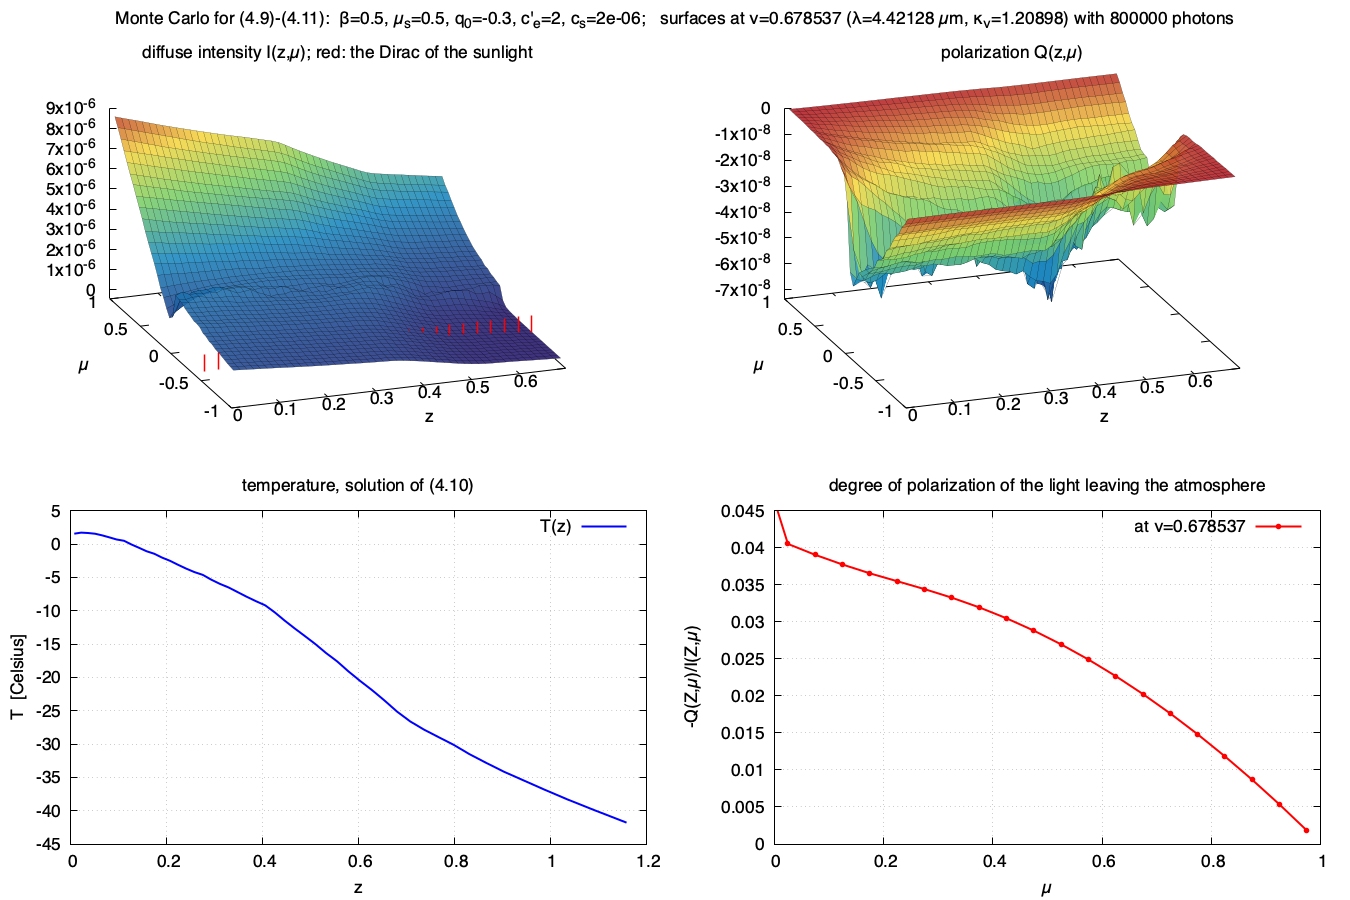
\includegraphics[height=0.74\textheight]{MCIQ4.png}
\end{center}
\vspace{-2mm}
{\scriptsize $Z=0.696$ (12 km), 554 frequencies, $\beta=0.5$, $\mu_s=0.5$, $q_0=-0.3$,
$T_e=291$K, $T_s=5778$K. The emerging light is polarized by 4\% at grazing angles, not at
all at the vertical --- no closure hypothesis.}
\end{frame}

%--------------------------------------------------------------------
\begin{frame}{Effect of CO$_2$: $\kappa_\nu\times1.2$ in the band 14--18\,$\mu$m}
\vspace{-2mm}
\begin{center}
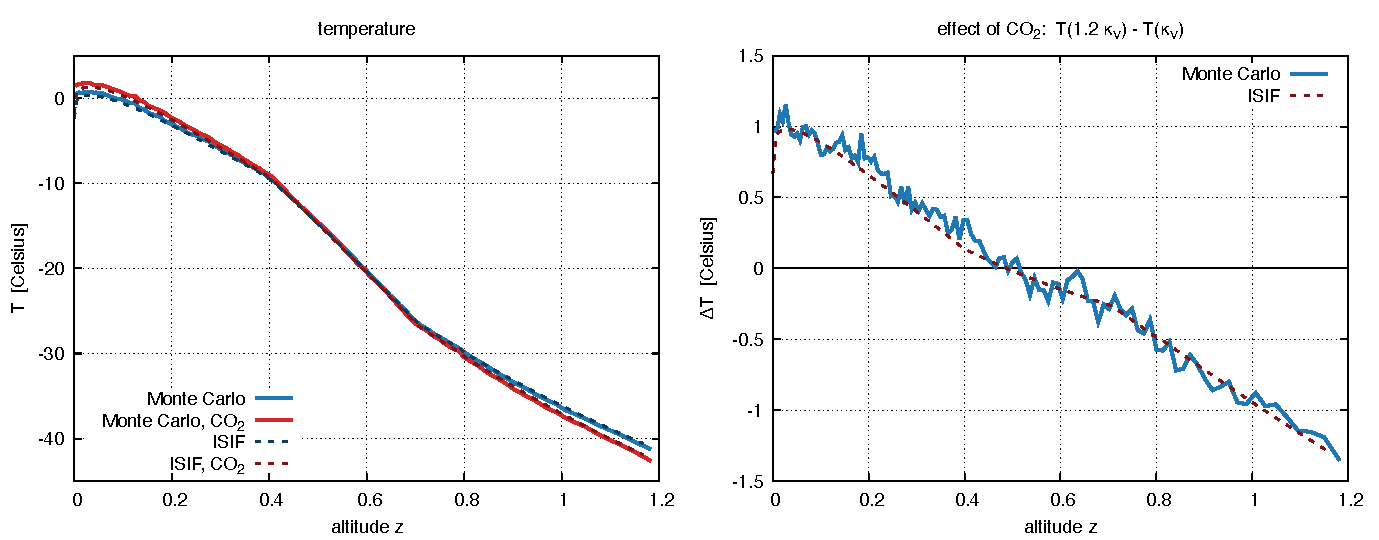
\includegraphics[width=0.76\textwidth]{compareISIF2MC.pdf}
\end{center}
\vspace{-4mm}
\begin{columns}[T]
\begin{column}{0.52\textwidth}
\begin{block}{The greenhouse signature}
\centering\footnotesize
\begin{tabular}{lrr}\toprule
& ground & tropopause\\ \midrule
Monte Carlo & $+0.97$ & $-1.35$\\
ISIF        & $+0.93$ & $-1.31$\\\bottomrule
\end{tabular}
\end{block}
\end{column}
\begin{column}{0.46\textwidth}
\footnotesize Both methods on the same 120 point grid. They agree on the \emph{signal} to
$0.2\,^\circ$C --- better than on $T$ itself: the systematic part of the discretization
error cancels in the difference. The $\pm0.1\,^\circ$C wiggle is the statistical error left
in a difference of two independent runs.
\end{column}
\end{columns}
\end{frame}

%--------------------------------------------------------------------
\begin{frame}{Cost of the three methods}
Same problem for the three: 554 frequencies, the CO$_2$ case, 25 temperature iterations,
on an Apple M4 Pro.
\begin{center}
\begin{tabular}{lrr}\toprule
& 49 cells & 119 cells\\\midrule
discrete ordinates \ \small(\texttt{SNIQ4.cpp}, 64 directions) & 0.64 s & 1.65 s\\
ISIF \ \small(\texttt{IQ4.cpp}) & 1.06 s & 5.96 s\\
Monte Carlo \ \small(\texttt{MCIQ4.cpp}, $2\cdot10^4$ photons per frequency) & 47 s & 102 s\\
\bottomrule
\end{tabular}
\end{center}
\medskip

Discrete ordinates: $9.4$ source iterations per frequency and per temperature iteration at
the tolerance $10^{-8}$; 64 directions give the ground temperature to $0.005\,^\circ$C. It
is the fastest of the three and the more so as the mesh is refined --- its cost is
$O(nN_z)$, against the $O(N_z^2)$ of the convolutions of ISIF.
\medskip

\begin{block}{Monte Carlo is not competitive in speed on this 1D problem}
Its interest is elsewhere: it needs neither the closure by the four moments
$J_0,J_2,K_0,K_2$, nor the exponential integrals $\E_n$, nor the fact that the kernel is a
polynomial in $\mu^2$. A phase matrix of any shape, a non stratified geometry or a non grey
ground would be taken unchanged --- and the frequencies are independent, hence trivially
parallel.
\end{block}
\end{frame}

%--------------------------------------------------------------------
\begin{frame}{The three methods give the same temperature}
\vspace{-2mm}
\begin{center}
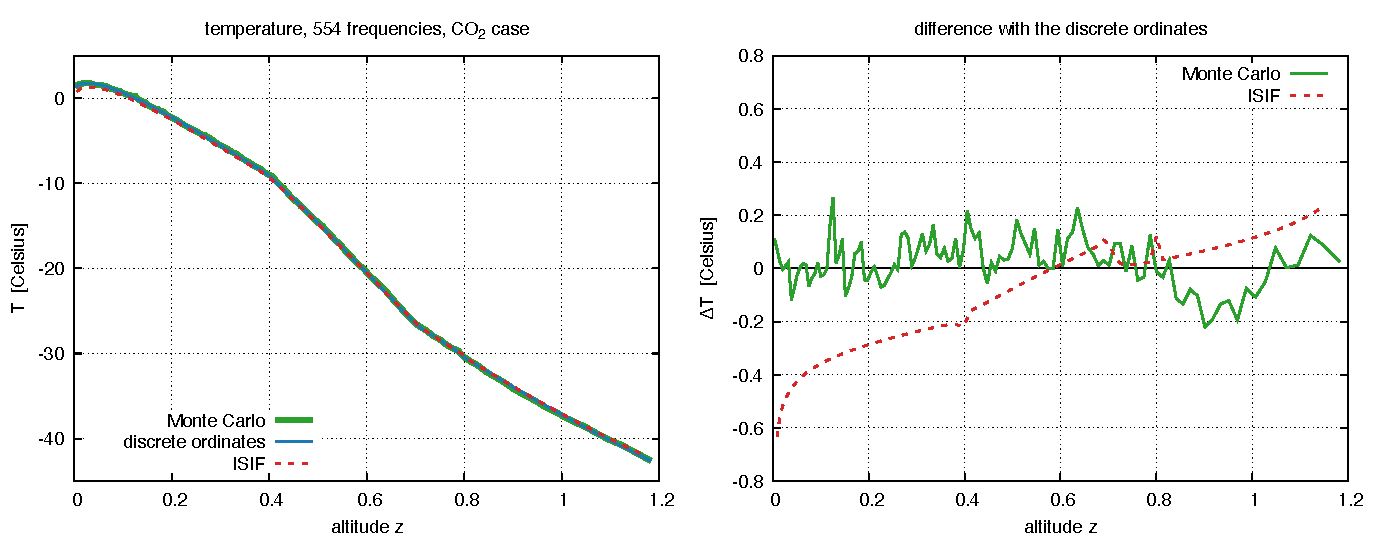
\includegraphics[width=0.84\textwidth]{compare3methods.pdf}
\end{center}
\vspace{-3mm}
\begin{columns}[T]
\begin{column}{0.46\textwidth}
\centering\footnotesize
\begin{tabular}{lrr}\toprule
difference with S$_N$ & max & r.m.s.\\\midrule
Monte Carlo & $0.27$ & $0.09$\\
ISIF        & $0.63$ & $0.24$\\\bottomrule
\end{tabular}
\end{column}
\begin{column}{0.52\textwidth}
\footnotesize Left: indistinguishable at this scale. Right: the Monte Carlo oscillates
about zero without trend --- statistical noise, decreasing like $N^{-1/2}$ --- while ISIF
departs smoothly and systematically, $-0.6\,^\circ$C at the ground, $+0.2\,^\circ$C at the
tropopause.
\end{column}
\end{columns}
\end{frame}

%--------------------------------------------------------------------
\begin{frame}{Conclusion}
\begin{itemize}
\item In the variables $I_l,I_r$ the scattering kernel of the VRTE is a
\emph{probability density}: a polarized radiative transfer problem can be simulated with
nonnegative weights.
\item Carrying $(w_l,w_r)$ and updating it deterministically removes the sampling noise on
$Q$ --- without it the method would be unusable.
\item Verified to $0.05\%$ on $J_0$ against discrete ordinates, and to $0.27\,^\circ$C
r.m.s.\ against ISIF.
\item A 20\% increase of $\kappa_\nu$ in the CO$_2$ band warms the ground by
$0.97\,^\circ$C and cools the tropopause by $1.35\,^\circ$C.
\end{itemize}
\vfill
{\footnotesize\textbf{Acknowledgement.} The programs --- the Monte Carlo solver \MC\ and
the discrete ordinates solver written to verify it --- together with the figures, the memo
and these slides, were produced by Claude Code (Anthropic, model Opus~5), from the
equations of Chapter~4 and the existing ISIF program \ISIF.}
\end{frame}

%--------------------------------------------------------------------
\begin{frame}{References}
\footnotesize
\begin{itemize}\itemsep3pt
\item J.~M. Hammersley, D.~C. Handscomb, {\em Monte Carlo Methods}, Methuen, 1964.
\item J.~Spanier, E.~M. Gelbard, {\em Monte Carlo Principles and Neutron Transport
Problems}, Addison-Wesley, 1969.
\item G.~I. Marchuk, G.~A. Mikhailov, M.~A. Nazaraliev et al., {\em The Monte Carlo
Methods in Atmospheric Optics}, Springer, 1980.
\item B.~Mayer, {\em Radiative transfer in the cloudy atmosphere}, EPJ Web of Conferences,
1 (2009), 75--99.
\item S.~Chandrasekhar, {\em Radiative Transfer}, Dover, 1960.
\item K.~Stamnes, S.-C. Tsay, W.~Wiscombe, K.~Jayaweera, {\em Numerically stable algorithm
for discrete-ordinate-method radiative transfer\dots}, Applied Optics, 27 (1988),
2502--2509.
\item E.~E. Lewis, W.~F. Miller, {\em Computational Methods of Neutron Transport}, Wiley,
1984.
\item M.~F. Modest, {\em Radiative Heat Transfer}, 3rd ed., Academic Press, 2013.
\end{itemize}
\end{frame}

\end{document}
